\subsection{Proof}
\begin{namedframe}{Proof of tangent chord theorem}
	\footnotesize
	\begin{proof}[Proof that $\angle TCA = \angle PTA$.]
		\begin{columns}
			\begin{column}{0.3\textwidth}
				\scriptsize
				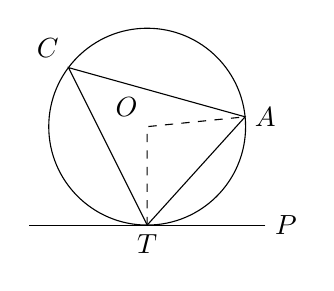
\begin{tikzpicture}[scale=0.25]
					\coordinate [label=above left:$O$](O) at (0,0);
					\coordinate [label=right:$P$](P) at (6,-5);
					\coordinate [label=below:$T$](T) at (0,-5);
					\coordinate (E) at (-6,-5);
					\coordinate [label=right:$A$](A) at (4.975, 0.499374608886);
					\coordinate [label=above left:$C$](C) at (-4, 3);

					\draw (O) circle (5);
					\draw (P) -- (T) -- (E);
					\draw (A) -- (C) -- (T) -- cycle;

					\uncover<2->{\draw [dashed] (T) -- (O) -- (A);}

					\uncover<4->{\tkzMarkRightAngle[size=0.75](O,T,P);}
				\end{tikzpicture}
			\end{column}
			\begin{column}{0.6\textwidth}
				We know that:
				\pause
				\begin{align*}
					2\angle ATO &= \SI{180}{\degree} - \angle AOT\\
					\angle ATO &= \frac{1}{2}(\SI{180}{\degree} - \angle AOT)
				\end{align*}
			\end{column}
		\end{columns}
		\pause
		We know from the Star Trek theorem that $\angle AOT = 2 \angle TCA$.
		\sep
		We also know that $\angle PTA = \SI{90}{\degree} - \angle ATO$.
		\sep
		We put this all together:
		\begin{align*}
			\uncover<+->{\angle PTA &= \SI{90}{\degree} - \frac{1}{2}(\SI{180}{\degree} - 2\angle TCA)\\}
			\uncover<+->{\angle PTA &= \SI{90}{\degree} - \SI{90}{\degree} + \angle TCA\\}
			\uncover<+->{\angle PTA &= \angle TCA \qedhere}
		\end{align*}
	\end{proof}
\end{namedframe}
